\documentclass[10pt,letterpaper]{article}\usepackage[]{graphicx}\usepackage[]{color}
%% maxwidth is the original width if it is less than linewidth
%% otherwise use linewidth (to make sure the graphics do not exceed the margin)
\makeatletter
\def\maxwidth{ %
  \ifdim\Gin@nat@width>\linewidth
    \linewidth
  \else
    \Gin@nat@width
  \fi
}
\makeatother

\definecolor{fgcolor}{rgb}{0.345, 0.345, 0.345}
\newcommand{\hlnum}[1]{\textcolor[rgb]{0.686,0.059,0.569}{#1}}%
\newcommand{\hlstr}[1]{\textcolor[rgb]{0.192,0.494,0.8}{#1}}%
\newcommand{\hlcom}[1]{\textcolor[rgb]{0.678,0.584,0.686}{\textit{#1}}}%
\newcommand{\hlopt}[1]{\textcolor[rgb]{0,0,0}{#1}}%
\newcommand{\hlstd}[1]{\textcolor[rgb]{0.345,0.345,0.345}{#1}}%
\newcommand{\hlkwa}[1]{\textcolor[rgb]{0.161,0.373,0.58}{\textbf{#1}}}%
\newcommand{\hlkwb}[1]{\textcolor[rgb]{0.69,0.353,0.396}{#1}}%
\newcommand{\hlkwc}[1]{\textcolor[rgb]{0.333,0.667,0.333}{#1}}%
\newcommand{\hlkwd}[1]{\textcolor[rgb]{0.737,0.353,0.396}{\textbf{#1}}}%
\let\hlipl\hlkwb

\usepackage{framed}
\makeatletter
\newenvironment{kframe}{%
 \def\at@end@of@kframe{}%
 \ifinner\ifhmode%
  \def\at@end@of@kframe{\end{minipage}}%
  \begin{minipage}{\columnwidth}%
 \fi\fi%
 \def\FrameCommand##1{\hskip\@totalleftmargin \hskip-\fboxsep
 \colorbox{shadecolor}{##1}\hskip-\fboxsep
     % There is no \\@totalrightmargin, so:
     \hskip-\linewidth \hskip-\@totalleftmargin \hskip\columnwidth}%
 \MakeFramed {\advance\hsize-\width
   \@totalleftmargin\z@ \linewidth\hsize
   \@setminipage}}%
 {\par\unskip\endMakeFramed%
 \at@end@of@kframe}
\makeatother

\definecolor{shadecolor}{rgb}{.97, .97, .97}
\definecolor{messagecolor}{rgb}{0, 0, 0}
\definecolor{warningcolor}{rgb}{1, 0, 1}
\definecolor{errorcolor}{rgb}{1, 0, 0}
\newenvironment{knitrout}{}{} % an empty environment to be redefined in TeX

\usepackage{alltt}
\usepackage[top=0.85in,left=2.75in,footskip=0.75in]{geometry}


\usepackage{amsmath,amssymb}

% Use adjustwidth environment to exceed column width (see example table in text)
\usepackage{changepage}

% Use Unicode characters when possible
\usepackage[utf8x]{inputenc}

% textcomp package and marvosym package for additional characters
\usepackage{textcomp,marvosym}

% cite package, to clean up citations in the main text. Do not remove.
\usepackage{cite}

% Use nameref to cite supporting information files (see Supporting Information section for more info)
\usepackage{nameref,hyperref}

% line numbers
\usepackage[right]{lineno}

% ligatures disabled
\usepackage{microtype}
\DisableLigatures[f]{encoding = *, family = * }

% color can be used to apply background shading to table cells only
\usepackage[table]{xcolor}

% array package and thick rules for tables
\usepackage{array}

% create "+" rule type for thick vertical lines
\newcolumntype{+}{!{\vrule width 2pt}}

% create \thickcline for thick horizontal lines of variable length
\newlength\savedwidth
\newcommand\thickcline[1]{%
  \noalign{\global\savedwidth\arrayrulewidth\global\arrayrulewidth 2pt}%
  \cline{#1}%
  \noalign{\vskip\arrayrulewidth}%
  \noalign{\global\arrayrulewidth\savedwidth}%
}

% \thickhline command for thick horizontal lines that span the table
\newcommand\thickhline{\noalign{\global\savedwidth\arrayrulewidth\global\arrayrulewidth 2pt}%
\hline
\noalign{\global\arrayrulewidth\savedwidth}}


% Remove comment for double spacing
%\usepackage{setspace}
%\doublespacing

% Text layout
\raggedright
\setlength{\parindent}{0.5cm}
\textwidth 5.25in
\textheight 8.75in

% Bold the 'Figure #' in the caption and separate it from the title/caption with a period
% Captions will be left justified
\usepackage[aboveskip=1pt,labelfont=bf,labelsep=period,justification=raggedright,singlelinecheck=off]{caption}
\renewcommand{\figurename}{Fig}

% Use the PLoS provided BiBTeX style
\bibliographystyle{plos2015}

% Remove brackets from numbering in List of References
\makeatletter
\renewcommand{\@biblabel}[1]{\quad#1.}
\makeatother



% Header and Footer with logo
\usepackage{lastpage,fancyhdr,graphicx}
\usepackage{epstopdf}
%\pagestyle{myheadings}
\pagestyle{fancy}
\fancyhf{}
%\setlength{\headheight}{27.023pt}
%\lhead{\includegraphics[width=2.0in]{PLOS-submission.eps}}
\rfoot{\thepage/\pageref{LastPage}}
\renewcommand{\headrulewidth}{0pt}
\renewcommand{\footrule}{\hrule height 2pt \vspace{2mm}}
\fancyheadoffset[L]{2.25in}
\fancyfootoffset[L]{2.25in}
\lfoot{\today}

%% Include all macros below

\newcommand{\lorem}{{\bf LOREM}}
\newcommand{\ipsum}{{\bf IPSUM}}

%% own packages
%% \usepackage[numbers]{natbib}
%% \usepackage{amsmath,mathtools,amssymb,mathrsfs,dsfont,amsthm}
%% \usepackage{caption}
%% \usepackage[T1]{fontenc}
%% \usepackage{babel}
%% \usepackage{graphicx}
%% \usepackage{float}
%% \usepackage{color}
\usepackage{subcaption}
%% \graphicspath{ {figs/} }
%% \usepackage{enumitem}
%% \usepackage{authblk}
%% \usepackage{lineno}
%% \usepackage[normalem]{ulem}

%% \usepackage{float}
%% \usepackage[nomarkers,figuresonly,nolists]{endfloat}
\IfFileExists{upquote.sty}{\usepackage{upquote}}{}
\begin{document}
\vspace*{0.2in}

% Title must be 250 characters or less.
\begin{flushleft}
{\Large
\textbf\newline{A bayesian mixture modelling approach for spatial proteomics}
}
\newline
%%
\\
Oliver M. Crook\textsuperscript{1,2,3},
Claire M. Mulvey\textsuperscript{2},
Paul D.W. Kirk\textsuperscript{3},
Kathryn S. Lilley\textsuperscript{2},
Laurent Gatto\textsuperscript{1,2\textcurrency *}
\\
\bigskip
\textbf{1} Computational Proteomics Unit, Department of  Biochemistry, University of Cambridge, Cambridge, UK
\\
\textbf{2} Cambridge Centre for Proteomics, Department of Biochemistry, University of Cambridge, Cambridge, UK
\\
\textbf{3} MRC Biostatistics Unit, Cambridge Institute for Public   Health, Cambridge, UK
\\
\bigskip


\textcurrency Current Address: de Duve Institute, UCLouvain, Avenue  Hippocrate 75, 1200 Brussels, Belgium

* laurent.gatto@uclouvain.be



\end{flushleft}
% Please keep the abstract below 300 words
\section*{Abstract}
Analysis of the spatial sub-cellular distribution of proteins is of
vital importance to fully understand context specific protein
function. Some proteins can be found with a single location within a
cell, but up to half of proteins may reside in multiple locations, can
dynamically re-localise, or reside within an unknown functional
compartment. These considerations lead to uncertainty in associating a
protein to a single location. Currently, mass spectrometry (MS) based
spatial proteomics relies on supervised machine learning algorithms to
assign proteins to sub-cellular locations based on common gradient
profiles. However, such methods fail to quantify uncertainty
associated with sub-cellular class assignment. Here we reformulate the
framework on which we perform statistical analysis. We propose a
Bayesian generative classifier based on Gaussian mixture models to
assign proteins probabilistically to sub-cellular niches, thus
proteins have a probability distribution over sub-cellular locations,
with Bayesian computation performed using the expectation-maximisation
(EM) algorithm, as well as Markov-chain Monte-Carlo (MCMC). Our
methodology allows proteome-wide uncertainty quantification, thus
adding a further layer to the analysis of spatial proteomics. Our
framework is flexible, allowing many different systems to be analysed
and reveals new modelling opportunities for spatial proteomics. We
find our methods perform competitively with current state-of-the art
machine learning methods, whilst simultaneously providing more
information. We highlight several examples where classification based
on the support vector machine is unable to make any conclusions, while
uncertainty quantification using our approach provides biologically
intriguing results.  To our knowledge this is the first Bayesian model
of MS-based spatial proteomics data.

\section*{Author summary}

Sub-cellular localisation of proteins provides insights into
sub-cellular biological processes. For a protein to carry out its
intended function it must be localised to the correct sub-cellular
environment, whether that be organelles, vesicles or any sub-cellular
niche. Correct sub-cellular localisation ensures the biochemical
conditions for the protein to carry out its molecular function are
met, as well as being near its intended interaction
partners. Therefore, mis-localisation of proteins alters cell
biochemistry and can disrupt, for example, signalling pathways or
inhibit the trafficking of material around the cell. The sub-cellular
distribution of proteins is complicated by proteins that can reside in
multiple micro-environments, or those that move dynamically within the
cell. Methods that predict protein sub-cellular localisation often
fail to quantify the uncertainty that arises from the complex and
dynamic nature of the sub-cellular environment. Here we present a
Bayesian methodology to analyse protein sub-cellular localisation. We
explicitly model our data and use Bayesian inference to quantify
uncertainty in our predictions. We find our
method is competitive with state-of-the-art machine learning methods
and additionally provides uncertainty quantification. We show that, with this
additional information, we can make deeper insights into the
fundamental biochemistry of the cell.



\section*{Introduction}\label{Intro}

Spatial proteomics is an interdisciplinary field studying the
localisation of proteins on a large-scale. Where a protein is
localised in a cell is a fundamental question, since a protein must be
localised to its required sub-cellular compartment to interact with
its binding partners (for example, proteins, nucleic acids, metabolic
substrates) and carry out its function
\cite{Gibson:2009}. Furthermore, mis-localisations of proteins are
also critical to our understanding of biology, as aberrant protein
localisation have been implicated in many pathologies
\cite{Olkkonen:2006, Luheshi:2008, Laurila:2009, De:2011, Cody:2013},
including cancer \cite{Kau:2004, Rodriguez:2004, Latorre:2005,
  Shin:2013} and obesity \cite{Siljee:2018}.

Sub-cellular localisations of proteins
can be studied by high-throughput mass spectrometry (MS)
\cite{Gatto:2010}. MS-based spatial proteomics experiments enable us
to confidently determine the sub-cellular localisation of thousands of
proteins within in a cell \cite{hyper}, given the availability of
rigorous data analysis and interpretation \cite{Gatto:2010}.

In a typical MS-based spatial proteomics experiment, cells first
undergo lysis in a fashion which maintains the integrity of their
organelles. The cell content is then separated using a variety of
methods, such as density separation \cite{Dunkley:2006,hyper},
differential centrifugation \cite{Itzhak:2016}, free-flow
electrophoresis \cite{Parsons:2014}, or affinity purification
\cite{Heard:2015}. In LOPIT \cite{Dunkley:2004, Dunkley:2006,
  Sadowski:2006} and \textit{hyper}LOPIT \cite{hyper,Mulvey:2017}, cell
lysis is proceeded by separation of the content along a density
gradient. Organelles and macro-molecular complexes are thus
characterised by density-specific profiles along the gradient
\cite{DeDuve:1981}.  Discrete fractions along the continuous density
gradient are then collected, and quantitative protein profiles that
match the organelle profiles along the gradient, are measured using
high accuracy mass spectrometry \cite{Mulvey:2017}.

The data are first visualised using principal component analysis (PCA)
and known sub-cellular compartments are annotated
\cite{ghrepo}. Supervised machine learning algorithms are then
typically employed to create classifiers that associate un-annotated
proteins to specific organelles \cite{Gatto:2014b}, as well as
semi-supervised methods that detect novel sub-cellular clusters using
both labelled and un-labelled features \cite{Breckels:2013}. More
recently, a state-of-the-art transfer learning (TL) algorithm has been
shown to improve the quantity and reliability of sub-cellular protein
assignments \cite{Breckels:2016}. Applications of such methods have
led to organelle-specific localisation information of proteins in
plants \cite{Dunkley:2006}, \textit{Drosophila} \cite{Tan:2009},
chicken \cite{hall:2009}, human cell lines \cite{Breckels:2013},
mouse pluripotent embryonic stem cells \cite{hyper} and cancer cell
lines \cite{Thul:2017}.

Classification methods which have previously been used include partial
least squares discriminate analysis \cite{Dunkley:2006}, K nearest
neighbours \cite{Groen::2014}, random forests \cite{Ohta::2010},
naive Bayes \cite{Nikolovski::2012}, neural networks
\cite{Tardif::2012} and the support vector machine amongst others
(see \cite{Gatto:2014b} for an overview). Although these methods have
proved successful within the field they have limitations. Typically,
such classifiers output an assignment of proteins to discrete
pre-annotated sub-cellular locations. However, it is important to note
that half the proteome cannot be robustly assigned to a single
sub-cellular location, which may be a manifestation of proteins in so
far uncharaterised organelles or proteins that are distributed amongst
multiple locations. These factors lead to uncertainty in the
assignment of proteins to sub-cellular localisations, and thus
quantifying this uncertainty is of vital importance \cite{Kirk:2015}.

To overcome the task of uncertainty quantification, this article
presents a probabilistic generative model for MS-based spatial
proteomics data. Our model posits that each annotated sub-cellular
niche can be modelled by a multivariate Gaussian distribution. Thus,
the full complement of annotated proteins is captured by a mixture of
multivariate Gaussian distributions. With the prior knowledge that
many proteins are not captured by known sub-cellular niches, we
augment our model with an outlier component. Outliers are often
dispersed and thus this additional component is described by a
heavy-tailed distribution: the multivariate Student's t-distribution,
leading us to a T Augmented Gaussian Mixture model (TAGM).

Given our model and proteins with known location, we can
probabilistically infer the sub-cellular localisation of thousands of
proteins. We can perform inference in our model by finding
\textit{maximum a posteriori} (MAP) estimates of the parameters. This
approach returns the probability of each protein belonging to each
annotated sub-cellular niche. These posterior localisation
probabilities can then be the basis for classification. In a more
sophisticated, fully Bayesian approach to uncertainty quantification,
we can additionally infer the entire posterior distribution of
localisation probabilities. This allows the uncertainty in the
parameters in our model to be reflected in the posterior localisation
probabilities. We perform this inference using Markov-chain
Monte-Carlo methods; in particular, we provide an efficient collapsed
Gibbs sampler to perform inference.

We perform a comprehensive comparison to state-of-the-art classifiers
to demonstrate that our method is reliable across $19$ different
spatial proteomics datasets and find that all classifiers we
considered perform competitively. To demonstrate the additional
biological advantages our method can provide, we apply our method to a
\textit{hyper}LOPIT dataset on mouse pluripotent embryonic stem cells
\cite{hyper}. We consider several examples of proteins that were
unable to be assigned using traditional machine-learning classifiers
and show that, by considering the full posterior distribution of
localisation probabilities, we can draw meaningful biological results
and make powerful conclusions. We then turn our hand to a more global
perspective, visualising uncertainty quantification for over 5,000
proteins, simultaneously. This approach reveals global patterns of
protein organisation and their distribution across sub-cellular
compartments.

We make extensive use of the R programming language \cite{R} and
existing MS and proteomics packages \cite{MSnbase:2012,
  pRoloc:2014}. We are highly committed to creating open software
tools for high quality processing, visualisation, and analysis of
spatial proteomics data.  We build upon an already extensive set of
open software tools \cite{pRoloc:2014} as part of the Bioconductor
project \cite{Bioconductor::2004, Huber::2015} and our methods are
made available as part of this project.

\section*{Results}

\subsection*{Application to mouse pluripotent embryonic stem cell data}

We model mouse pluripotent embryonic stem cell (E14TG2a) data
\cite{hyper}, which contains quantitation data for $5032$
proteins. This high-resolution map was produced using the
\textit{hyper}LOPIT workflow \cite{Mulvey:2017}, which uses a
sophisticated sub-cellular fractionation scheme. This fractionation
scheme is made possible by the use of Tandem Mass Tag (TMT) 10-plex
and high accuracy TMT quantification was facilitated by using
synchronous precursor selection MS3 (SPS-MS3) \cite{Mcalister::2014},
which reduces well documented issues with ratio distortion in
isobaric multiplexed quantitative proteomics \cite{Ting:2011}. The
data resolves $14$ sub-cellular niches with an additional chromatin
preparation resolving the nuclear chromatin and non-chromatin
components. Two biological replicates of the data are concatenated,
each with $10$ fractions along the density gradient. {\color{black}{We defined gold
standard organelle markers as those with unambiguous single annotation
\cite{Gatto:2014b}. A protein marker list for the mouse pluripotent embryonic
stem cells was manually curated using information from the UniProt database,
the Gene Ontology and the literature, as was performed in \cite{hyper}}}. The following
section applies our statistical methodology to these data and we
explore the results.

\subsubsection*{Maximum a posteriori prediction of protein localisation}

This section applies the TAGM model to the mouse pluripotent embryonic
stem cell data, by deriving MAP estimates for the model parameters and
using these for prediction.  Visualisation is important for data
analysis and exploration. A simple way to visualise our model is to
project probability ellipses onto a PCA plot. Each ellipse contains a
proportion of total probability of a particular multivariate Gaussian
density.  The outer ellipse contains $99\%$ of the total probability
whilst the middle and inner ellipses contain $95\%$ and $90\%$ of the
probability respectively. Visualising only the first two principal
components can be misleading, since proteins can be more (or less)
separated in subsequent principal components.  We visualise the first
two principal components along with the first and fourth principal
components as a representative example. For the TAGM model, we derive
probability ellipses from the MAP estimates of the parameters (figure
\ref{figure::pcaellipse}).




\begin{figure}[!p]
  \begin{subfigure}[t]{0.45\textwidth}
    \centering

\end{subfigure}%
\hfill
\begin{subfigure}[t]{0.45\textwidth}
        \centering

\end{subfigure}
  \centering
  \caption{ (a) PCA plot of the 1st and 2nd principal components for
    the curated marker proteins of the mouse stem cell data. The
    organelles are, in general, well separated. Though some organelles
    overlap, they are separated along different principal
    components. The densities used to produce the ellipses are derived
    from the MAP estimates. (b) Marker resolution along the 1st and
    4th principal components show that the mitochondrion and
    peroxisome markers are well resolved, despite overlapping in the
    1st and 2nd component.  We also see that the ER/Golgi apparatus
    markers are better separated from the extracellular matrix
    markers.}
\label{figure::pcaellipse}
\end{figure}


We now apply the statistical methodology described in section
\nameref{section:methods}, to predict the localisation of proteins to
organelles and sub-cellular components. In brief, we produce MAP
estimates of the parameters by using the expectation-maximisation
algorithm, to form the basis of a Bayesian analysis (TAGM-MAP).  We
run the algorithm for $200$ iterations and inspect a plot of the
log-posterior to assess convergence of the algorithm (see supporting
information, section S3). We confirm that the difference of the log
posterior between the final two iterations is less than $10^{-6}$ and
we conclude that our algorithm has converged. The results can be seen
in figure \ref{fig:assignmentPCA} (left), where the posterior
localisation probability is visualised by scaling the pointer for each
protein.

Figure \ref{fig:assignmentPCA} (right) demonstrates a range of
probabilistic assignments of proteins to organelles and sub-cellular
niches. We additionally consider a full, sampling-based Bayesian
analysis using Markov-chain Monte Carlo (MCMC) to characterise the
uncertainty in the localisation probabilities.  In our case a
collapsed Gibbs sampler is used to sample from the posterior of
localisation probabilities. The remainder of this article focus on
analysis of spatial proteomics in this fully Bayesian framework.




\subsubsection*{Uncertainty in the posterior localisation probabilities}

This section applies the TAGM model to the mouse pluripotent embryonic
stem cell data, by considering the uncertainty in the parameters and
exploring how this uncertainty propogates to the uncertainty in
protein localisation prediction.  In figure
\ref{figure::pcaellipseMCMC} we visualise the model as before using
the first two principal components along with the first and fourth
principal component as a representive example.  For the TAGM model, we
derive probability ellipses from the expected value of the posterior
normal-inverse-Wishart (NIW) distribution.

We apply the statistical methodology detailed in section
\nameref{section:methods}.  We perform posterior computation in the
Bayesian setting using standard MCMC methods (TAGM-MCMC).  We run $6$
chains of our Gibbs sampler in parallel for $15,000$ iterations,
throwing away the first $4,000$ iterations for burn-in and retain
every $10^{th}$ sample for thinning.  Thus 1,100 sample are retained
from each chain. We then visualise the trace plots of our chains; in
particular, we monitor the number of proteins allocated to the known
components (see supporting information, section S4). We discard $1$ chain because
we do not consider it to have converged.  For the remaining $5$
chains we further discard the first $500$ samples by visual
inspection.  We then have $600$ retained samples from $5$ separate
chains. For further analysis, we compute the Gelman-Rubin convergence
diagnostic \cite{Gelman:1992, Brooks:1998}, which is computed as
$\hat{R} \approx 1.05$.  Values of $\hat{R}$ far from 1 indicate
non-convergence and since our statistic is less than $1.1$, we
conclude our chains have converged. The remaining samples are then
pooled to produce a single chain containing $3000$ samples.

We produce point estimates of the posterior localisation probabilities
by summarising samples by their Monte-Carlo average.  These summmaries
are then visualised in figure \ref{fig:assignmentPCA} (right panel),
where the pointer {\color{black}{is scaled according to the localisation
probabilities of the sub-cellular niche with the largest posterior
probability}}. Monte-Carlo based inference also provides us with
additional information; in particular, we can interrogate individual
proteins and their posterior probability distribution over
sub-cellular locations.

Figure \ref{fig:G5E870} illustrates one example of the importance of
capturing uncertainty.  The E3 ubiquitin-protein ligase TRIP12
(G5E870) is an integral part of ubiquitin fusion degradation pathway
and is a protein of great interest in cancer because it regulates DNA
repair pathways. The SVM failed to assign this protein to any
location, with assigment to the 60S Ribosome falling below a $5\%$ FDR
and the MAP estimate assigned the protein to the nucleus non-chromatin
with posterior probability < 0.95.  The posterior distribution of
localisation probabilities inferred from the TAGM-MCMC model, shown in
figure \ref{fig:G5E870}, demonstrates that this protein is most
probably localised to the nucleus non-chromatin. However, there is
some uncertainty about whether it localises to the $40$S ribosome.
This could suggest a dynamic role for this protein, which could be
further explored with a more targeted experiment.



\subsubsection*{Enrichment analysis of outlier proteins}

In previous sections, we demonstrated that we can assign proteins
probabilitically to sub-cellular compartment and quantify the
uncertainty in these assignments. Some proteins cannot be well
described as belonging to any known component and we model this
using an additional T-distribution outlier component
{\color{black}{(see Section \nameref{section:methods})}}.

It is biologically interesting to decipher what functional role
proteins that are far away from known components play. We perform an
over-representation analysis of gene ontology (GO) terms to asses the
biological relevance of the outlier component \cite{Boyle:2004,
  Yu:2012}. We take 1111 proteins that were allocated to known
components with probability less than $0.95$.  Note that these 1111
proteins exclude proteins that are likely to belong to a known
location, but we are uncertain about which localisation.  We then
perform enrichment analysis against the set of all proteins
quantified in the \textit{hyper}LOPIT experiment. We search against
the cellular compartment, biological process and molecular function
ontologies.

Supplementary figure 3 shows this outlier component
is enriched for cytoskeletal part ($p <10^{-7}$) and microtuble
cytoskeleton ($p <10^{-7}$). Cytoskeleton proteins are found
throughout the cell and therefore we would expect them to be found in
every fraction along the density gradient. We also observe enrichment
for highly dynamic sub-cellular processes such as cell division
($p <10^{-6}$) and cell cycle processes ($p <10^{-6}$), again these
proteins are unlikely to have steady-state locations within a single
component. We also see enrichment for molecular functions such as
tranferase activity $(p < 0.005)$, another highly dynamic
process. These observations justify including an additional outlier
component in our mixture model.

\subsection*{Comparison with other classifiers}

In this section, we assess the generalisation performance of our
methods on several datasets, by computing performance metrics
associated with each classifier as detailed in section
\nameref{section::assessment}. We compare the SVM and KNN classifiers
alongside the MAP and MCMC approaches detailed in the methods
section. We compute the F1 score and quadratic loss over 100 rounds of
stratified 5-fold cross-validation. The hyperparameter for the KNN
algorithm, the number of nearest neighbours, is optimised via an
additional internal 5-fold cross-validation and the hyperparameters
for the SVM, sigma and cost, are also optimised via internal 5-fold
cross validation \cite{svm:2010}.

We test our methods on the following datasets \textit{Drosophila}
\cite{Tan:2009}, chicken \cite{hall:2009}, mouse pluripotent
embryonic stem cells from \cite{hyper} and \cite{Breckels:2016}, the
human bone osteosarcoma epithelial (U2-OS) cell line
\cite{Thul:2017}, the HeLa cell line of \cite{Itzhak:2016}, the $3$
HeLa cell lines from \cite{Hirst:2018} and $10$ primary fibroblast
datasets from \cite{Jean_Beltran:2016}.  These datasets represent a
great variety of spatial proteomics experiments across many different
workflows.

The two \textit{hyper}LOPIT datasets on mouse pluripotent embryonic
stem cells and the U2-OS cell line use TMT 10-plex labelling and
contain the greatest number of proteins.  Earlier LOPIT experiments on
the \textit{Drosophila} and chicken use iTRAQ 4-plex labelling, whilst
another LOPIT mouse pluripotent embryonic stem cell dataset uses iTRAQ
8-plex. The datasets of \cite{Itzhak:2016} and \cite{Hirst:2018}
employ a different methodology completely - seperating cellular
content using differential centrifugation (as opposed to along a
density-gradient).  Furthermore, the methods use SILAC rather than
iTRAQ or TMT for labelling. The experiments of \cite{Hirst:2018} were
designed to explore the functional role of AP-5 by coupling
CRISPR-CAS9 knockouts with spatial proteomics methods. We analysed all
three datasets from \cite{Hirst:2018}, which includes a wild type HeLa
cell line as a control, as well as two CRISPR-CAS9 knockouts:
AP5Z1-KO1 and AP5Z1-KO2 respectively.

In addition, we analyse the spatio-temporal proteomics experiments of
\cite{Jean_Beltran:2016}, which uses TMT-based MS quantification. This
experiment explored infecting primary fibroblasts with Human
cytomegalovirus (HMCV) and the goal of these experiments was to
explore the dynamic perturbation of host proteins during infection, as
well as the sub-cellular localisation of viral proteins throught the
HCMV life-cycle. They produced spatial maps at different time points:
$24,48,72,96,120$ hours post infection (hpi), as well as mock maps at
these same time points to serve as a control - this results in $10$
different spatial proteomics maps.

In each case, a dataset specific marker list was used, which is
curated specifically for the each cell line. We removed
"high-curvature ER" annotations from the HeLa dataset
\cite{Itzhak:2016}, as well as the "ER Tubular", "Nuclear pore
complex" and "Peroxisome" annotations from the HeLa CRISPR-CAS9
knockout experiments \cite{Hirst:2018} as there are too few proteins
to correctly perform cross-validation. Table \ref{table:data}
summarises these datasets, including information about number of
quantified proteins, the workflow used and the number of fractions.

\begin{table}[h]
\centering
\begin{tabular}{ |p{3cm}|p{3cm}|p{2cm}|p{2cm}|p{2cm}|  }
 \hline

 \multicolumn{5}{|c|}{MS-based Spatial Proteomics datasets} \\
 \hline
 Cell line or organism & Workflow & Labelling & Fractions (including combined replicates) & Proteins \\
 \hline
 \hline
 \textit{Drosophila}   &  LOPIT & iTRAQ & 4  & 888\\
 \hline
 Chicken DT40 & LOPIT  & iTRAQ & 16 & 1090 \\
 \hline
 Mouse pluripotent E14TG2a stem cell  &  HyperLOPIT & TMT & 20 & 5032\\
 \hline
 HeLa (Itzhak et al.) & Organeller Maps & SILAC & 30 & 3766\\
 \hline
 HeLa (Hirst et al.) & Organeller Maps  & SILAC & 15 & 2046\\
 \hline
 U2-OS cell line & HyperLOPIT  & TMT & 37 & 5020\\
 \hline
 Primary Fibroblast & Spatio-Temporal Methods & TMT & 6 & 2196 \\
 \hline
 E14TG2a (Breckels et al.)  &  LOPIT & iTRAQ & 8 & 2031\\
\hline
\end{tabular}
\caption{Summary of spatial proteomics datasets used for comparisons}
\label{table:data}
\end{table}

Figure \ref{figure::f1scores} compares the Macro-F1 scores across the
datasets for all classifiers and demonstrates that no single
classifier consistently outperforms any other across all datasets,
with results being highly consistent across all methods, as well as
across datasets. We perform a pairwise unpaired t-test with multiple
testing correction applied using the Benjamini-H\"ochberg procedure
\cite{FDR:1995} to detect differences between classifier performance.

In the \textit{Drosophila} dataset only the KNN algorithm outpeforms
the SVM at significance level of $0.01$, whilst no other significant
differences exist between the classifiers. In the chicken DT40 dataset
only the MCMC method outperforms the KNN classifier at significance
level of $0.01$, no other significant conclusion can be drawn. In the
mouse dataset the MAP based method outperforms the MCMC method at
significance level of $0.01$, no other significant conclusions can be
drawn. In the HeLa dataset all classifiers are significantly different
at a $0.01$ level. These differences may exist because the dataset does
not fit well with our modelling assumptions; in particular, this
dataset set has been curated to have a class called "Large Protein
Complex", which likely describes several sub-cellular
structures. These might include nuclear compartments and ribosomes, as
well as any cytosolic complex and large protein complex which pellets
during the centrifugation conditions used to capture this mixed
sub-cellular fraction. Moreover, the cytosolic and nuclear fraction
were processed separately leading to possible imbalance with
comparisions with other datasets. Thus, the large protein complex
component might be better described as itself a mixture model or more
detailed curation of these data may be required. We do not consider
further modelling of this dataset in this manuscript. For the U2-OS
all classifiers are significantly different at a significance level of
$0.01$ except for the SVM classifier and the MCMC method, with the MAP
method performing the best. Figure \ref{figure::f1scores} shows that
for this dataset all classifiers are performing extremely well. In the
three Hirst datasets the MAP method significantly outperforms all
other methods $(p < 0.01)$, whilst in the wild type HeLa and in the
CRISPR-CAS9 KO1 there is no significant difference between the KNN
and MCMC method. In the CRISPR-CAS9 KO2 the MCMC method outperforms
the SVM and KNN methods $(p < 0.01)$. In the interest of brevity, the
remaining results for the t-tests can be found in tables in supporting information, section S5.





The Macro-F1 scores do not take into account that whilst the TAGM
model may misclassify, it may do so with low confidence. We therefore
additionally compute the quadratic loss, which allows us to make use
of the probabilitic information provided by the classifiers. The lower
the quadratic loss the closer the probabilitic predicition is to the
true value. We plot the distributions of quadratic losses for each
classifier in figure \ref{figure::quadloss}. We observe highly
consitent performance across all classifiers across all
datasets. Again, we perform a pairwise unpaired t-test with multiple
testing correction.

We find that in 16 out of 19 datasets {\color{black}{(all of those except HeLa Wild type,
HeLa KO1 and HeLa KO2)}} the MCMC methods achieves the
lowest quadratic loss at a signifiance level $<0.0001$ over the SVM
and KNN classifiers. In 6 out of these 16 datasets there is no
significant difference between the MCMC and the MAP methods. In the
three Hirst datasets in which the MCMC did not acheive the lowest
quadratic loss, the SVM outperformed. However, in two of these
datasets (HeLa Wild type and KO1) the MAP method and SVM classifier were
not significantly different. In the Hirst KO2 dataset there were no
signicant differences between the MAP and MCMC methods.

In the vast majority of cases, we observe that if the TAGM model,
using the MCMC methodology, makes an incorrect classification it does
so with lower confidence than the SVM classifier, the KNN classifier
and the MAP based classifier, whilst if it is correct in its assertion
it does so with greater confidence. Additionally, a fully Bayesian
methodology provides us with not only point estimates of
classification probabilities but uncertainty quantification in these
allocations, and we show in the following section that this provides
deeper insights into protein localisation.





Computing distributions of F1 scores and quadratic losses, which can
only be done on the marker proteins, can help us understand whether a
classifier might have greater generalised performance
accuracy. However, we are interested in whether there is a large
disagreement between classifiers when prediction is performed on
proteins for which we have no withheld localisation information. This
informs us about a systematic bias for a particular classifier or
whether a classifier ensemble could increase performance. To maintain
a common set of proteins we set thresholds for each classifier in turn
and compare to the other classifier without thresholding. Firstly, we
set a global threshold of 0.95 for the TAGM-MCMC and then for these
proteins plot a contingency table against the classification results
from the SVM. Secondly, we set a 5\% FDR for the SVM and then for
these proteins plot a contingency table against the classification
results from the TAGM-MCMC. We visualise the contingency tables as
heat plots in figure \ref{figure:contigencytables}.





In general, we see an extremely high level of coherence between the
TAGM and the SVM, with almost all proteins predicted to concordant
sub-cellular compartments. Figure \ref{figure:contigencytables} shows
there is some disagreement between assigning proteins to the lysosome
and plasma membrane, to the cytosol and proteasome, and between the
large and small ribosomal subunits.  However, we have not used the
uncertainty in the probabilitic assignments to produce the contingency
tables above. In the next sections, we explore examples of proteins
with uncertainty in their posterior localisation
probabilities. Selecting biologically relevant thresholds is important
for any classifier and exploring uncertainty is of vital importance
when drawing biological conclusions.


\subsection*{Interpreting and exploring uncertainty}

Protein sub-cellular localisation can be uncertain for a number of
reasons. Technical variations and unknown biological novelty, such as
yet uncharacterised functional compartments, can be some of the
reasons why a protein might have an unknown or uncertain
localisation. Furthermore many proteins are known to reside in
multiple locations with possibly different functional duties in each
location \cite{Jeffery:2009}. With these considerations in mind, it is pertinent to
quantify the uncertainty in our allocation of proteins to organelles.
This section explores several situations where proteins display
uncertain localisation and considers the biological factors that
influence uncertainty.  We later explore and visualise whole proteome
uncertainty quantification.

\bigskip

Exportin 5 (Q924C1) forms part of the micro-RNA export machinery of
the nucleus, transporting miRNA from the nucleus to the cytoplasm for
further processing.  It then translocates back through the nuclear
pore complex to return to the nucleus.  Exportin 5 can then continue
to mediate further transport between nucleus and cytoplasm.  The SVM
was unable to assign a localisation of Exportin 5, with its assignment
falling below a $5\%$ FDR to wrongly assign this protein to the
proteasome. This incorrect assertion by the SVM was confounded by the
similarity between the cytosol and proteasome profiles.  Figure
\ref{fig:Q924C1} demonstrates, according to the TAGM-MCMC model, that
Exportin 5 most likely localises to the cytosol but there is some
uncertainty with this assignment.  This uncertainty is reflected in
possible assignment of Exportin 5 to the nucleus non-chromatin and
this uncertainty is a manifestation of the the fact that the function
of this protein is to shuttle between the cytosol and nucleus.

The Phenylalanine--tRNA ligase beta subunit protein (Q9WUA2) has an
uncertain localisation between the 40S ribosome and the nucleus
non-chromatin demonstrated in figure \ref{fig:Q9WUA2}. This protein
was left unclassified by the SVM because its score fell below a $5\%$
FDR threshold to assign it to the 40S ribosome. Considering that this
protein is involved in the acylation of transfer RNA (tRNA) with the
amino acid phenylalanine to form tRNA--Phe to be used in translation of
proteins, it is therefore unsurprising that this protein's steady
state location is ribosomal.  Whilst the SVM is unable to make an
assignment, TAGM-MCMC is able to suggest an assignment and quantify our
uncertainty.

Relatively little is known about the Dedicator of cytokinesis (DOCK)
protein 6 (Q8VDR9), a guanine nucleotide exchange factor for CDC42 and
RAC1 small GTPases. The SVM could not assign localisation to the
ER/Golgi, since its score fell below a $5\%$ FDR. Furthermore, the
TAGM-MCMC model assigned this DOCK 6 to the outlier component with
posterior probability $>0.95$.  Figure \ref{fig:Q8VDR9} shows possible
localisation to several components along the secretory pathway. As an
activator for CDC42 and RAC1 we may expect to see them with similar
localisation. CDC42, a plasma membrane associated protein, regulates
cell cycle and division and is found with many
localisations. Furthermore RAC1, a small GTPase, also regulates many
cellular processes and is found in many locations. Thus the
steady-state distribution of DOCK6 is unlikely to be in a single
location, since its interaction partners are found in many
locations. This justifies including an outlier component in our model,
else we may erroneously assign such proteins to a single location.




\subsection*{Visualising whole sub-cellular proteome uncertainty}

The advantage of the TAGM-MCMC model is its ability to provide
proteome wide uncertainy quantification. Regions where organelle
assignments overlap are areas were uncertainty is expected to be the
greatest, as well as areas with no dominant component. We take an
information theoretic approach to summarising uncertainty in protein
localisation by computing the Shannon entropy \cite{shannon:1948} for
each Monte-Carlo sample $t = 1,...,T$ of the posterior localisation
probabilities of each protein

\begin{equation}
\left\{H^{(t)} = - \sum_{k=1}^Kp^{(t)}_{ik} \log\left(p^{(t)}_{ik}\right)\right\}^{T}_{t=1},
\end{equation}

where $p^{(t)}_{ik}$ denotes the posterior localisation probabilty of
protein $i$ to component $k$ at iteration $t$. We then summarise this
as a Monte-Carlo averaged Shannon entropy.  The greater the Shannon
entropy the more uncertainty associated with the assignment of this
protein. The lower the Shannon entropy the lower the uncertainty
associated with the assignment of this protein.  In figure
\ref{figure:proteomeuncertainty} panel (a), we visualise the Shannon
entropy of each protein in a PCA plot, by scaling the pointers in
accordance to this metric. We also note that while localisation
probability (of a protein to its most probable location) and the
Shannon entropy are correlated, figure
\ref{figure:proteomeuncertainty} panel (c), it is not perfect. Thus it
is important to use both the localisation probabilities and the
uncertainty in these assignments to make conclusions.


Figure \ref{figure:proteomeuncertainty} demonstrates that the regions
of highest uncertainty are those in regions where organelles
assignments overlap. The conclusions from this plot are
manifold. Firstly, many proteins are assigned unambiguously to
sub-cellular localisations; that is, not only are some proteins
assigned to organelles with high probability but also with low
uncertainty. Secondly, there are well defined regions with high
uncertainty, for example proteins in the secretory pathway or proteins
on the boundary between cytosol and proteasome. Finally, some
organelles, such as the mitochondria, are extremely well
resolved. This observed uncertainty in the secretory pathway and
cytosol could be attributed to the dynamic nature of these parts of
the cell with numerous examples of proteins that traffic in and out of
these sub-cellular compartments as part of their biological
role. Moreover, the organelles of the secretory pathway share similar
and overlapping physical properties making their separation from one
another using biochemical fractionation more challenging.
Furthermore, there is a region located in the centre of the plot where
proteins simultaneously have low probability of belonging to any
organelle and high uncertainty in their localisation probability.
This suggests that these proteins are poorly described by any single
location. These proteins could belong to multiple locations or belong
to undescribed sub-cellular compartments. The information displayed in
these plots and the conclusion therein would be extremely challenging
to obtain without the use of Bayesian methodology.


\section*{Discussion}

We have demonstrated that a Bayesian framework, based on Gaussian
mixture models, for spatial proteomics can provide whole sub-cellular
proteome uncertainty quantification on the assignment of proteins to
organelles and such information is invaluable. Performing MAP
inference using our generative model provides fast and straightforward
approach, which is vital for quality control and early data
exploration. Full posterior inference using MCMC provides not only
point estimates of the posterior probability that a protein belongs to
a particular sub-cellular niche, but uncertainty in this
assignment. Then, this uncertainty can be summarised in several ways,
including, but not limited to, equi-tailed credible intervals of the
Monte-Carlo samples of posterior localisation probabilities.
Posterior distributions for indivdual proteins can then be rigorously
interrogated to shed light on their biological mechanisms; such as,
transport, signalling and interactions.

As well as the local uncertainty seen by exploring individual
proteins, we further explored using a Monte-Carlo averaged Shannon
entropy to visualise global uncertainty. Regions of high uncertainty,
as measured using this Shannon entropy, reflect highly dynamics
regions of the sub-cellular environment.  Hence, biologists can now
explore uncertainty at different levels and then are able to make
quantifiable conclusions and insights about their data.  Furthermore,
our Bayesian model is interpretable and our inferences are fully
conditional on our data, allowing them to be easily modified with
changing experimental design.

In addition, we produced competitive classifier performance to the
state-of-the-art classifiers. We considered two traditional
machine-learning methods: the SVM and KNN classifiers; as well as two
classifiers based on our model: a MAP classifier and classification
based on MCMC. We compared all methods on 19 different spatial
proteomics datasets, across four different organisms. When considering
the macro-F1 score as a performance metric, no single classifier
outperformed another across all datasets. However, using MCMC based
inference our method significantly outperforms the SVM and KNN
classifiers with respect to the quadratic loss in $16$ our of $19$
datasets. This allows us to have greater confidence in our conclusions
when they are draw from our Bayesian inferences. Furthermore, using
MCMC provides a wealth of additional information, and so becomes the
method of choice for analysing spatial proteomics data.

Analysis of a \textit{hyper}LOPIT experiment applied to mouse
pluripotent embryonic stem cells demonstrated that the additional
layer of information that our model provides is biologically relevant
and provides further avenues for additional exploration. Moreover,
applying our method to a biologically significant dataset now provides
the scientific community with localisation information on up to 4000
proteins for the mouse pluripotent stem cell proteome. Figure
\ref{figure:ConcludePlot} demonstrates that from an initial input of
roughly 1000 marker proteins with \textit{a priori} known location and
4000 unknown proteins with unknown location, SVM and TAGM-MCMC can
provide rigorous localisation information on roughly 2000
proteins. However, our methodology, by also considering uncertainty,
allows us to obtain information on another 1000 proteins. Thus, we
have augmented this dataset by providing uncertainty quantification on
the localisation of proteins to their sub-cellular niches, which had
been previously unavailable.
{\color{black}{We note that our method is general enough
to be applied to many MS-based spatial proteomics protocols including:
LOPIT, \textit{hyper}LOPIT, protein correlation profiling (PCP) \cite{Foster:2006},
differential centrifugation approaches and spatio-temporal proteomics methods.
In our flexible software implementation, all hyperparameters for the priors can be
changed if users have precise priors they wish to specify.}}



We have also provided a new set of visualisation methods to accompany
our model, which allow us to easily interrogate our data. High quality
visualisation tools are essential for rigorous quality control and
sound biological conclusions.  Our methods have been developed in the
R statistical programming language and we continue to contribute to
the Bioconductor project \cite{Bioconductor::2004, Huber::2015} with
inclusion of our methods within the pRoloc package ($>=$ 1.21.1)
\cite{pRoloc:2014}. The underlying source code used to generate this
document is available at
\url{https://github.com/lgatto/2018-TAGM-paper}.

\bigskip

%% \sout{Currently, our model cannot integrate localisation information from
%% different data sources nor can it explicity model proteins with
%% multiple localisation. In addition, extensions to semi-supervised
%% methods are under consideration to detect novel sub-cellular
%% niches. These are the subjects of further work.}

{\color{black}{Currently, our model does not integrate localisation information
from different data sources, nor does it explicitly model proteins with multiple
localisation. However, one (of many) biological explanations for the uncertainty
that we model in the allocation probabilities is provided by multiple localisation.
Thus a protein for which it is uncertain to which two sub-cellular niches it is
resident within it is perhaps resident of both niches. In further work, we plan
to explicitly model such cases to deconvolute different sources of uncertainty.
In addition, extensions to semi-supervised non-parametric methods are under
consideration to detect novel sub-cellular niches. These are the subjects of further work.
}}


\bigskip

\section*{Model}\label{section:methods}

We describe in this section the probabilistic model that uses the
labelled data to associate un-annotated proteins to specific
organelles or sub-cellular compartments.

\subsection*{Mixture models for spatial proteomic data}

We observe $N$ protein profiles each of length $L$, corresponding to
the number of quantified fractions along the gradient density,
including combining replicates.  For $i = 1, \ldots, N$, we denote the
profile of the $i$-th protein by
${\bf x}_i = [x_{1i}, \ldots, x_{Li}]$.  We suppose that there are $K$
known sub-cellular compartments to which each protein could localise
(e.g. cytoplasm, endoplasmic reticulum, mitochondria, \ldots).
Henceforth, we refer to these $K$ sub-cellular compartments as {\em
  components}, and introduce component labels $z_i$, so that $z_i = k$
if the $i$-th protein localises to the $k$-th component. We denote by
$X_L$ the set of proteins whose component labels are known, and by
$X_U$ the set of unlabelled proteins.  If protein $i$ is in $X_U$, we
desire the probability that $z_i = k$ for each $k = 1, \ldots, K$.
That is, for each unlabelled protein, we want the probability of
belonging to each component (given a model and the observed data).


We initially model the distribution of profiles associated with
proteins that localise to the $k$-th component as multivariate normal
with mean vector $\boldsymbol{\mu}_k$ and covariance matrix
$\Sigma_k$, so that:

\begin{align}
{\bf x}_i | z_i = k \quad \sim \mathcal{N}(\boldsymbol{\mu}_k, \Sigma_k). \label{equation::preq}
\end{align}

For any $i$, we define the prior probability of the $i$-th protein
localising to the $k$-th component to be $p(z_i = k) = \pi_k$.
Letting
$\boldsymbol{\theta} = \{\boldsymbol{\mu}_k, \Sigma_k \}_{k = 1}^K$
denote the set of all component mean and covariance parameters, and
$\boldsymbol{\pi} = \{\pi_k\}_{k = 1}^K$ denote the set of all mixture
weights, it follows (from the law of total probability) that:

\begin{align}
p({\bf x}_i | \boldsymbol{\theta}, \boldsymbol{\pi} ) = \sum_{k = 1}^K \pi_k f({\bf x}_i|\boldsymbol{\mu}_k, \Sigma_k),\label{equation::mmeq}
\end{align}

where $f({\bf x} | \boldsymbol{\mu}, \Sigma)$ denotes the density of
the multivariate normal with mean vector $\boldsymbol{\mu}$ and
covariance matrix $\Sigma$ evaluated at ${\bf x}$.

Equation \eqref{equation::mmeq} defines a generative probabilistic
model known as a {\em mixture model}.  Such models are useful for
describing populations that are composed of a number of distinct
homogeneous subpopulations.  In our case, we model the full complement
of measured proteins as being composed of $K$ subpopulations, each
corresponding to a different organelle or sub-cellular
compartment. The literature of mixture model applications to biology
is rich and some recent example include applications to retroviral
integration sites \cite{Kirk:2016}, genome-wide associations studies
\cite{Liley:2017}, single-cell transcriptomics
\cite{Lonnberg:2017} {\color{black}{and affinity purification MS proteomics}}
\cite{Choi:2010}.

Though some proteins are well described as belonging to a single
component, many proteins multi-localise or might belong to
uncharacterised organelles. In order to allow the model to better
account for these "outliers" that cannot be straightforwardly
allocated to any single known component, we extend it by introducing
an additional "outlier component". To do this, we augment our model by
introducing a further indicator latent variable $\phi$. Each protein
${\bf x}_i$ is now described by an additional variable $\phi_i$, with
$\phi_i = 1$ indicating that protein ${\bf x}_i$ belongs to a
organelle derived component and $\phi_i = 0$ indicating that protein
${\bf x}_i$ is not well described by these known components. This
outlier component is modelled as a multivariate T distribution with
degrees of freedom $\kappa$, mean vector $\bf{M}$, and scale matrix
$V$. Thus equation \eqref{equation::preq} becomes

\begin{align}
{\bf x}_i | z_i = k, \phi_i \quad \sim \mathcal{N}(\boldsymbol{\mu}_k, \Sigma_k)^{\phi_i}\mathcal{T}(\kappa, \boldsymbol{M}, V)^{1 - \phi_i }.
\end{align}

Further let $g({\bf x | \kappa, \bf{M}, V} )$ denote the density of
the multivariate T-distribution so that Equation
\eqref{equation::mmeq} becomes:

\begin{equation} \label{equation::tammeq}
  \begin{split}
    p({\bf x}_i| \boldsymbol{\theta}, \boldsymbol{\pi} ,\phi_i, \kappa, {\bf M}, V) &=  \sum_{k=1}^{K}\pi_k\left(f({\bf x}_i|\boldsymbol{\mu}_k, \Sigma_k)^{\phi_i}g({\bf x}_i|\kappa, \boldsymbol{M}, V)^{1 - \phi_i }\right).\\
  \end{split}
\end{equation}

For any $i$, we define the prior probability of the $i$-th protein
belonging to the outlier component as $p(\phi_i = 0) = \epsilon$.

We can then rewrite equation \eqref{equation::tammeq} in the following way:

\begin{equation}\label{equation::tammepseq}
  \begin{split}
    p({\bf x}_i| \boldsymbol{\theta}, \boldsymbol{\pi} , \kappa, \epsilon, {\bf M}, V) &=  \sum_{k=1}^{K}\pi_k\left((1-\epsilon)(f({\bf x}_i |\boldsymbol{\mu}_k, \Sigma_k) + \epsilon g({\bf x}_i|\kappa, \boldsymbol{M}, V)\right),\\
  \end{split}
\end{equation}

Throughout we take $\kappa = 4$, ${\bf M}$ as the global mean, and $V$
as half the global variance of the data, {\color{black}{including labelled and unlabelled proteins}}.
The reason for formulating
the model as in equation \eqref{equation::tammeq} is because it leads
to a flexible modelling framework. Furthermore, $\phi$ has an elegant
model selection interpretation, since it decides whether ${\bf x}_i$
is better modelled by the known components or the outlier component.
It is important to note that $f$ and $g$ could be replaced by many
combinations of distributions and thus could be valuable in modelling
other datasets. The choice of parameters for the multivariate
T-distribution was decided so that it mimicked a multivariate normal
component with the same mean and variance but with heavier tails to
better capture dispersed proteins, which we refer to as outlier
proteins throughout the text. {\color{black}{The variance of the multivariate T-distribution
is designed to be large such that is relatively flat when compared with multivariate Gaussian
distributions which describe annotated components. }} Similar approaches for modelling
outliers have been explored in the literature and often the outlier
term is considered constant or as a Poisson process, independent of
the observation \cite{Banfield::1993, Cooke::2011, Coretto::2016,
  Hennig::2004}.


\subsection*{Model fitting}

We adopt a Bayesian approach toward inferring the unknown parameters,
$\boldsymbol{\theta} = \{\boldsymbol{\mu}_k, \Sigma_k \}_{k = 1}^K$,
$\boldsymbol{\pi} = \{\pi_k\}_{k = 1}^K$, and $\epsilon$ of the
mixture model presented in Equation \eqref{equation::tammeq}.  For
$\boldsymbol{\pi}$, we take a conjugate symmetric Dirichlet prior with
parameter~$\beta$, so that
$\pi_1, \ldots, \pi_K \sim \mbox{Dirichlet}(\beta)$; and for the
component-specific parameters $\boldsymbol{\mu}_k$ and $\Sigma_k$ we
take conjugate normal-inverse-Wishart (NIW) priors with parameters
$\{\boldsymbol{\mu}_0, \lambda_0, \nu_0, S_0\}$, so that:

\begin{equation} \label{equation::prior}
  \mu_k, \Sigma_k \quad \sim \mathcal{N}\left(\boldsymbol{\mu}_k|\boldsymbol{\mu}_0, \frac{\Sigma_{k}}{\lambda_0}\right)I\mathcal{W}\left(\Sigma_{k}|\nu_0, S_0\right).
\end{equation}

We also place a conjugate Beta prior on $\epsilon$ with parameters $u$
and $v$, so that $\epsilon \sim \mathcal{B}(u,v)$.  Allowing
$\epsilon$ to be random allows us to infer the number of proteins that
are better described by an outlier component rather than any known
component.

The full model, which we henceforth refer to as a T-augmented Gaussian
Mixture model (TAGM), can then be summarised by the plate diagram
shown in Figure \ref{plateDiagram}.


To perform inference for the parameters, we make use of both the
labelled and unlabelled data. For the labelled data $X_L$, since $z_i$
and $\phi_i$ are known for these proteins, we can update the
parameters with their data analytically by exploiting conjugacy of the
priors (see, for example \cite{Gelman:1995}). For the unlabelled
data we do not have such information and so in the next sections we
explain how to make inferences of the latent variables.

\subsection*{Prediction of localisation of unlabelled proteins}

Having obtained the posterior distribution of the model parameters
analytically using, at first, the labelled data only, we wish to
predict the component to which each of the unlabelled proteins
belongs. The probability that a protein belongs to any of the $K$
known components, that is $z_i = k$ and $\phi_i = 1$, is given by (see
supporting information section S1 for derivations):

\begin{equation}\label{equation::estep1}
\begin{split}
p(\phi_i = 1, z_i = k|{\bf x}_i, \boldsymbol{\theta}, \boldsymbol{\pi} , \epsilon,\kappa, {\bf M}, V)  & = \frac{\pi_k(1-\epsilon)f({\bf x}_i|\boldsymbol{\mu}_k, \Sigma_{k})}{\sum_{k=1}^{K}\pi_k\left((1-\epsilon) f({\bf x}_i|\boldsymbol{\mu}_k, \Sigma_k) + \epsilon g({\bf x}_i|\kappa, {\bf M}, V)\right)},
\end{split}
\end{equation}
whilst on the other hand,
\begin{equation}\label{equation::estep2}
\begin{split}
p(\phi_i = 0, z_i = k|{\bf x}_i, \boldsymbol{\theta}, \boldsymbol{\pi},\kappa, \epsilon, {\bf M}, V)  = \frac{\pi_k \epsilon g({\bf x}_i|\kappa, {\bf M}, V)}{\sum_{k=1}^{K}\pi_k\left((1-\epsilon) f({\bf x}_i|\boldsymbol{\mu}_k, \Sigma_k) + \epsilon g({\bf x}_i|\kappa, {\bf M}, V)\right)}.
\end{split}
\end{equation}

Processing of the unlabelled data can be done by inferring {\em maximum
  a posteriori} (MAP) estimates for the parameters. However, this
approach fails to account for the uncertainty in the parameters, thus
we additionally explore inferring the distribution over these
parameters.

\subsubsection*{Maximum a posteriori prediction}

We use the Expectation-Maximisation (EM) algorithm \cite{EM:1977} to
find {\em maximum a posteriori} (MAP) estimates for the parameters
(see, for example, \cite{Murphy:2012}). To specify the parameters of
the prior distributions, we use a simple set of heuristics provided by
\cite{Fraley:2007}. By defining the following quantities

\begin{equation}\label{equation::estepfinal}
\begin{split}
a_{ik} = & p(z_i = k, \phi_i = 1|{\bf x}_i), b_{ik} = p(z_i = k, \phi_i = 0|{\bf x}_i) \\
w_{ik} = & p(z_i = k|x_i) = a_{ik} + b_{ik}\\
a_k = & \sum_{i=1}^{n}a_{ik}, a = \sum_{k=1}^{K}a_k \\
b_k = & \sum_{i=1}^{n}b_{ik}, b = \sum_{k=1}^{K}b_k \\
r_k = & \sum_{i=1}^{n}w_{ik},
\end{split}
\end{equation}

we can compute

\begin{equation}\label{equation::Posterior}
\begin{split}
\lambda_k = &\lambda_0 + a_k, \\
\nu_k = & \nu_0 + a_k, \\
m_k = & \frac{a_k\bar{\boldsymbol{x}}_k + \lambda_0\mu_0}{\lambda_k},\\
S_k^{-1}  = & S_0^{-1} + \frac{\lambda_0 a_k}{\lambda_k}(\bar{\boldsymbol{x}}_k - \mu_0)^{T} (\bar{\boldsymbol{x}}_k - \mu_0) + \sum_{i=1}^{n} a_{ik}(x_i -\bar{\boldsymbol{x}}_k)^{T}(x_i -\bar{\boldsymbol{x}}_k).
\end{split}
\end{equation}

Then the parameters of the posterior mode are:

\begin{equation}\label{equation::MAP}
\begin{split}
\hat{{\bf\mu}}_k = &m_k \\
\hat{\Sigma}_k = &\frac{1}{\nu_k + D + 2}S_k^{-1}.
\end{split}
\end{equation}

We note if $\boldsymbol{x}_i$ is a labelled protein then $a_{ik} = 1$
and these parameters can be updated without difficulty.  The above
equation constitutes a backbone of the E-step of the EM algorithm, with
the entire algorithm specified by the following summary:


E-Step: Given the current parameters compute the values given by
equations (\ref{equation::estepfinal}), with formulae provided in
equations (\ref{equation::estep1}) and (\ref{equation::estep2}).

\bigskip

M-Step: Compute
\[\epsilon = \frac{ u + b - 1}{(a+b) + (u+v) - 2},\]
and
\[\pi_k = \frac{r_k + \beta_k - 1}{N + \sum \beta_k - K},\]
as well as
\[\bar{\boldsymbol{x}}_k = \frac{1}{a_k}\left(\sum_{i=i}^{n}a_{ik}{\bf x}_i\right).\]

Finally, compute the MAP estimates given by equations
(\ref{equation::MAP}). These estimates are then used in the following
iteration of the E-step.


Denoting by Q the expected value of the log-posterior and letting $t$
denote the current iteration of the EM algorithm, we iterate until
$\lvert Q(\boldsymbol{\theta}|\boldsymbol{\theta}_{t}) -
Q(\boldsymbol{\theta}|\boldsymbol{\theta}_{t-1})\rvert < \delta$ for
some pre-specified $\delta >0$.  Once we have found MAP estimates for
the parameters $\boldsymbol{\theta}_{MAP}$, $\boldsymbol{\pi}_{MAP}$
and $\epsilon_{MAP}$ we proceed to perform prediction. We plug the MAP
parameter estimates into Equation \eqref{equation::estep1} in order to
obtain the posterior probability of protein $i$ localising to
component $k$,
$p(z_i = k, \phi = 1 | {\bf x}_i, \boldsymbol{\theta}_{MAP},
\boldsymbol{\pi}_{MAP} , \epsilon_{MAP},\kappa, {\bf M}, V)$. To make
a final assignment, we may allocate each protein according to the
component that has maximal probability.  A full technical derivation
of the EM algorithm can be found in the supporting information (section S1).

\subsubsection*{Uncertainty in the posterior localisation probabilities}\label{section::MCMC}

The MAP approach described above provides us with a probabilistic
assignment,
$p(z_i = k, \phi = 1 | {\bf x}_i, \boldsymbol{\theta}_{MAP},
\boldsymbol{\pi}_{MAP} , \epsilon_{MAP},\kappa, {\bf M}, V)$, of each
unlabelled protein to each component.  However, it fails to account
for the uncertainty in the parameters $\boldsymbol{\theta}$,
$\boldsymbol{\pi}$ and $\epsilon$. To address this, we can sample
parameters from the posterior distribution.

Let
$\{\boldsymbol{\theta}^{(t)}, \boldsymbol{\pi}^{(t)},
\epsilon^{(t)}\}_{t=1}^T$ be a set of $T$ sampled values for the
parameters $\boldsymbol{\theta}$, $\boldsymbol{\pi}, \epsilon$, drawn
from the posterior.


The assignment probabilities can then be summarised by the Monte-Carlo
average:

\[p(z_i = k, \phi = 1 | {\bf x}_i, \epsilon, {\bf M}, V) \approx T^{-1}\sum_{t=1}^{T}p(z_i = k, \phi = 1 | {\bf x}_i, \boldsymbol{\theta}^{(t)}, \boldsymbol{\pi}^{(t)} , \epsilon^{(t)}, \kappa, {\bf M}, V).\]

Other summaries of the assignment probabilities can be determined in
the usual ways to obtain, for example, interval-estimates. We
summarise interval-estimates using the $95\%$ equi-tailed interval,
which is defined by the $0.025$ and $0.975$ quantiles of the
distribution of assignment probabilities,
$\{p(z_i = k, \phi = 1 | {\bf x}_i, \boldsymbol{\theta}^{(t)},
\boldsymbol{\pi}^{(t)} , \epsilon^{(t)}, {\bf M}, V) \}_{t=1}^T$.

Sampling parameter values in our model requires us to compute the
required conditional probabilities and then a straightforward Gibbs
sampler can be used to sample in turn from these conditionals. In
addition, we can bypass sampling the parameters by exploiting the
conjugacy of our priors. By marginalising parameters in our model we
can obtain an efficient collapsed Gibbs sampler and therefore only
sample the component allocation probabilities and the outlier
allocation probabilities. The derivations and required conditionals
can be found in the supporting information (section S2).

\subsection*{Classifier assessment}\label{section::assessment}

We compared the classification performance of the two
above learning schemes to the K-nearest neighbours (KNN) and the
weighted support vector machine (SVM) classifiers.

The following schema was used to assess the classifier performance of
all methods. We split the marker sets for each experiment into a
class-stratified training $(80\%)$ and test $(20\%)$ partitions, with
the separation formed at random. The true classes of the test profiles
are withheld from the classifier, whilst the algorithm is trained. The
algorithm is then assessed on its ability to predict the classes of
the proteins in the test partition for generalisation accuracy. How
each classifier is trained is specific to that classifier.  The KNN
and SVM have hyperparameters optimised using $5$-fold
cross-validation. This $80/20$ data stratification is performed $100$
times in order to produce $100$ sets of macro-F1 \cite{He::2009}
scores and class specific F1 scores \cite{Breckels:2016}. The F1
score is the harmonic mean of the precision and recall, more
precisely:
\[\text{precision}=\frac{tp}{tp+fp}, \text{recall} = \frac{tp}{tp+fn}.\]

tp denotes the number of true positives; fp the number of
false positives and fn the number of false negatives. Thus

\[\text{F1}=2\times\frac{\text{precision}\times\text{recall}}{\text{precision}+\text{recall}}.\]

High Macro F1 scores indicates that marker proteins in the test
dataset are consistently correctly assigned by the classifier. We note
that accuracy alone is an inadequate measure of performance, since it
fails to quantify false positives.

However, a Bayesian Generative classifier produces probabilistic
assignment of observations to classes. Thus while the classifier may
make an incorrect assignment it may do so with low probability. The F1
score is unforgiving in this situation and will not use this
information.  To measure this uncertainty, we introduce the quadratic
loss which allows us to compare probabilistic assignments
\cite{Gneiting:2007}.  For the SVM, a logistic distribution is fitted
using maximum likelihood estimation to the decision values of all
binary classifiers. Then, the membership probabilities for the
multi-class classification is calculated using quadratic optimisation.
The logistic regression model assumes errors which are distributed
according to a centred Laplace distribution for the predictions, where
maximum likelihood estimation is used to estimate the scale parameter
\cite{Meyer:2017}.  For the KNN classifier, we interpret the
proportion of neighbours belonging to each class as a non-parametric
posterior probability. To avoid non-zero probabilities for classes we
perform Laplace smoothing; that is, the posterior allocation
probability is given by

\begin{equation}
p(z_i = k|x_i) = \frac{N_{ik} + \alpha d_k C}{K + \alpha C},
\end{equation}

where $N_{ik}$ is the number of neighbours belonging to class $k$ in
the neighbourhood of $x_i$, $C$ is the number of classes, $K$ is the
number of nearest neighbours (optimised through 5-fold cross
validation) and $d_k$ is the incidence rate of each class in the
training set. Finally, $\alpha >0$ is the pseudo-count smoothing
parameter. Motivated by a Bayesian interpretation of placing a
Jeffrey's type Dirichlet prior over multinomial counts, we choose
$\alpha = 0.5$ \cite{Hazimeh:2015, Valcarce:2016, Manning:2008}.  The
quadratic loss is given by the following formula:

\begin{equation}
  Q_2 = \sum_{i = 1}^{N}\lVert q_i - p_i\rVert_2^2,
\end{equation}

where $\lVert\cdot\rVert_2$ is the $l_2$ norm and $q_i$ is the true
classification vector and $p_i$ is a vector of predicted assignments
to each class. It is useful to note that the corresponding risk
function is the mean square error (MSE), which is the expected value
of the quadratic loss.

%% Request from PLoS:
%%  Please remove the funding information from the manuscript and instead
%%  ensure that this information has been entered correctly into the
%%  Financial Disclosure section of the online submission form.

%% \subsection*{Funding}

%% LG was supported by the BBSRC Strategic Longer and Larger grant
%% (Award BB/L002817/1) and the Wellcome Trust Senior Investigator
%% Award 110170/Z/15/Z awarded to KSL. PDWK was supported by the MRC
%% (project reference MC\_UP\_0801/1). CMM was supported by a Wellcome
%% Trust Technology Development Grant (Grant number
%% 108467/Z/15/Z). OMC is a Wellcome Trust Mathematical Genomics and
%% Medicine student supported financially by the School of Clinical
%% Medicine, University of Cambridge. The funders had no role in study
%% design, data collection and analysis, decision to publish, or
%% preparation of the manuscript.


\subsection*{Acknowledgments}

The authors would also like to thank Dr Sean B. Holden, University of
Cambridge, for helpful discussions.


\begin{thebibliography}{99}

\bibitem{Gibson:2009}
Gibson T.
\newblock Cell regulation: determined to signal discrete cooperation.
\newblock Trends in biochemical sciences. 2009;34(10):471--482.

\bibitem{Olkkonen:2006}
Olkkonen V, Ikonen E.
\newblock When intracellular logistics fails-genetic defects in membrane
  trafficking.
\newblock Journal of cell science. 2006;119(24):5031--5045.

\bibitem{Luheshi:2008}
Luheshi L, Crowther D, Dobson C.
\newblock Protein misfolding and disease: from the test tube to the organism.
\newblock Current opinion in chemical biology. 2008;12(1):25--31.

\bibitem{Laurila:2009}
Laurila K, Vihinen M.
\newblock Prediction of disease-related mutations affecting protein
  localization.
\newblock BMC genomics. 2009;10(1):122.

\bibitem{De:2011}
De~Matteis M, Luini A.
\newblock Mendelian disorders of membrane trafficking.
\newblock New England Journal of Medicine. 2011;365(10):927--938.

\bibitem{Cody:2013}
Cody N, Iampietro C, L{\'e}cuyer E.
\newblock The many functions of mRNA localization during normal development and
  disease: from pillar to post.
\newblock Wiley Interdisciplinary Reviews: Developmental Biology.
  2013;2(6):781--796.

\bibitem{Kau:2004}
Kau T, Way J, Silver P.
\newblock Nuclear transport and cancer: from mechanism to intervention.
\newblock Nature Reviews Cancer. 2004;4(2):106--117.

\bibitem{Rodriguez:2004}
Rodriguez J, Au W, Henderson B.
\newblock Cytoplasmic mislocalization of BRCA1 caused by cancer-associated
  mutations in the BRCT domain.
\newblock Experimental cell research. 2004;293(1):14--21.

\bibitem{Latorre:2005}
Latorre I, Roh M, Frese K, Weiss R, Margolis B, Javier R.
\newblock Viral oncoprotein-induced mislocalization of select PDZ proteins
  disrupts tight junctions and causes polarity defects in epithelial cells.
\newblock Journal of cell science. 2005;118(18):4283--4293.

\bibitem{Shin:2013}
Shin S, Smith J, Rezniczek G, Pan S, Chen R, Brentnall T, et~al.
\newblock Unexpected gain of function for the scaffolding protein plectin due
  to mislocalization in pancreatic cancer.
\newblock Proceedings of the National Academy of Sciences.
  2013;110(48):19414--19419.

\bibitem{Siljee:2018}
Siljee J, Wang Y, Bernard A, Ersoy B, Zhang S, Marley A, et~al.
\newblock Subcellular localization of {MC4R} with {ADCY3} at neuronal primary
  cilia underlies a common pathway for genetic predisposition to obesity.
\newblock Nat Genet. 2018 Jan;.

\bibitem{Gatto:2010}
Gatto L, Vizca{\'\i}no J, Hermjakob K, Huber W, Lilley K.
\newblock Organelle proteomics experimental designs and analysis.
\newblock Proteomics. 2010;10(22):3957--3969.

\bibitem{hyper}
Christoforou A, Mulvey C, Breckels L, Geladaki A, Hurrell T, Hayward P, et~al.
\newblock A draft map of the mouse pluripotent stem cell spatial proteome.
\newblock Nature communications. 2016;7:9992.

\bibitem{Dunkley:2006}
Dunkley T, Hester S, Shadforth I, Runions J, Weimar T, Hanton S, et~al.
\newblock Mapping the Arabidopsis organelle proteome.
\newblock Proceedings of the National Academy of Sciences.
  2006;103(17):6518--6523.

\bibitem{Itzhak:2016}
Itzhak D, Tyanova S, Cox J, Borner G.
\newblock Global, quantitative and dynamic mapping of protein subcellular
  localization.
\newblock Elife. 2016;5:e16950.

\bibitem{Parsons:2014}
Parsons H, Fern{\'a}ndez-Ni{\~n}o S, Heazlewood J.
\newblock Separation of the plant Golgi apparatus and endoplasmic reticulum by
  free-flow electrophoresis.
\newblock Methods in molecular biology (Clifton, NJ). 2014;1072:527.

\bibitem{Heard:2015}
Heard W, Sklen{\'a}{\v{r}} J, Tome D, Robatzek S, Jones A.
\newblock Identification of regulatory and cargo proteins of endosomal and
  secretory pathways in Arabidopsis thaliana by proteomic dissection.
\newblock Molecular \& Cellular Proteomics. 2015;14(7):1796--1813.

\bibitem{Dunkley:2004}
Dunkley T, Watson R, Griffin J, Dupree P, Lilley K.
\newblock Localization of organelle proteins by isotope tagging (LOPIT).
\newblock Molecular \& Cellular Proteomics. 2004;3(11):1128--1134.

\bibitem{Sadowski:2006}
Sadowski P, Dunkley T, Shadforth I, Dupree P, Bessant C, Griffin J, et~al.
\newblock Quantitative proteomic approach to study subcellular localization of
  membrane proteins.
\newblock Nature protocols. 2006;1(4):1778--1789.

\bibitem{Mulvey:2017}
Mulvey C, Breckels L, Geladaki A, Britov{\v{s}}ek N, Nightingale D,
  Christoforou A, et~al.
\newblock Using {hyperLOPIT} to perform high-resolution mapping of the spatial
  proteome.
\newblock Nature Protocols. 2017;12(6):1110--1135.

\bibitem{DeDuve:1981}
De~Duve C, Beaufay H.
\newblock A short history of tissue fractionation.
\newblock The Journal of cell biology. 1981;91(3):293.

\bibitem{ghrepo}
Breckels L, Mulvey C, Lilley K, Gatto L.
\newblock A Bioconductor workflow for processing and analysing spatial
  proteomics data.
\newblock F1000Research. 2016;5.

\bibitem{Gatto:2014b}
Gatto L, Breckels L, Burger T, Nightingale D, Groen A, Campbell C, et~al.
\newblock A foundation for reliable spatial proteomics data analysis.
\newblock Molecular \& Cellular Proteomics. 2014;p. mcp--M113.

\bibitem{Breckels:2013}
Breckels L, Gatto L, Christoforou A, Groen A, Lilley K, Trotter M.
\newblock The effect of organelle discovery upon sub-cellular protein
  localisation.
\newblock Journal of proteomics. 2013;88:129--140.

\bibitem{Breckels:2016}
Breckels L, Holden S, Wojnar D, Mulvey C, Christoforou A, Groen A, et~al.
\newblock Learning from heterogeneous data sources: an application in spatial
  proteomics.
\newblock PLoS computational biology. 2016;12(5):e1004920.

\bibitem{Tan:2009}
Tan D, Dvinge H, Christoforou A, Bertone P, Martinez~Arias A, Lilley K.
\newblock Mapping organelle proteins and protein complexes in drosophila
  melanogaster.
\newblock Journal of proteome research. 2009;8(6):2667--2678.

\bibitem{hall:2009}
Hall S, Hester S, Griffin J, Lilley K, Jackson A.
\newblock The organelle proteome of the DT40 lymphocyte cell line.
\newblock Molecular \& Cellular Proteomics. 2009;8(6):1295--1305.

\bibitem{Thul:2017}
Thul P, Akesson L, Wiking M, Mahdessian D, Geladaki A, Ait~Blal H, et~al.
\newblock A subcellular map of the human proteome.
\newblock Science. 2017;.

\bibitem{Groen::2014}
Groen A, Sancho-Andres G, Breckels L, Gatto L, Aniento F, Lilley K.
\newblock Identification of trans-Golgi network proteins in Arabidopsis
  thaliana root tissue.
\newblock Journal of proteome research. 2014;13(2):763--776.

\bibitem{Ohta::2010}
Ohta S, Bukowski-Wills J, Sanchez-Pulido L, de~Lima~Alves F, Wood L, Chen Z,
  et~al.
\newblock The protein composition of mitotic chromosomes determined using
  multiclassifier combinatorial proteomics.
\newblock Cell. 2010;142(5):810--821.

\bibitem{Nikolovski::2012}
Nikolovski N, Rubtsov D, Segura M, Miles G, Stevens T, Dunkley T, et~al.
\newblock Putative glycosyltransferases and other plant Golgi apparatus
  proteins are revealed by LOPIT proteomics.
\newblock Plant physiology. 2012;160(2):1037--1051.

\bibitem{Tardif::2012}
Tardif M, Atteia A, Specht M, Cogne G, Rolland N, Brugi{\`e}re S, et~al.
\newblock {PredAlgo}: a new subcellular localization prediction tool dedicated
  to green algae.
\newblock Molecular biology and evolution. 2012;29(12):3625--3639.

\bibitem{Kirk:2015}
Kirk P, Babtie A, Stumpf M.
\newblock Systems biology (un) certainties.
\newblock Science. 2015;350(6259):386--388.

\bibitem{R}
{R Core Team}. R: A Language and Environment for Statistical Computing. Vienna,
  Austria; 2017.
\newblock Available from: \url{https://www.R-project.org/}.

\bibitem{MSnbase:2012}
Gatto L, Lilley K.
\newblock MSnbase - an R/Bioconductor package for isobaric tagged mass
  spectrometry data visualization, processing and quantitation.
\newblock Bioinformatics. 2012;28:288--289.

\bibitem{pRoloc:2014}
Gatto L, Breckels L, Wieczorek S, Burger Y, Lilley K.
\newblock Mass-spectrometry based spatial proteomics data analysis using pRoloc
  and pRolocdata.
\newblock Bioinformatics. 2014;.

\bibitem{Bioconductor::2004}
Gentleman R, Carey V, Bates D, Bolstad B, Dettling M, Dudoit S, et~al.
\newblock Bioconductor: open software development for computational biology and
  bioinformatics.
\newblock Genome biology. 2004;5(10):R80.

\bibitem{Huber::2015}
Huber W, Carey V, Gentleman R, Anders S, Carlson M, Carvalho B, et~al.
\newblock Orchestrating high-throughput genomic analysis with Bioconductor.
\newblock Nature methods. 2015;12(2):115.

\bibitem{Mcalister::2014}
McAlister G, Nusinow D, Jedrychowski M, W{\:u}hr M, Huttlin E, Erickson B, et~al.
\newblock MultiNotch MS3 enables accurate, sensitive, and multiplexed detection
  of differential expression across cancer cell line proteomes.
\newblock Analytical chemistry. 2014;86(14):7150--7158.

\bibitem{Ting:2011}
Ting L, Rad R, Gygi S, Haas W.
\newblock MS3 eliminates ratio distortion in isobaric multiplexed quantitative
  proteomics.
\newblock Nature methods. 2011;8(11):937.

\bibitem{Gelman:1992}
Gelman A, Rubin D.
\newblock Inference from iterative simulation using multiple sequences.
\newblock Statistical science. 1992;p. 457--472.

\bibitem{Brooks:1998}
Brooks S, Gelman A.
\newblock General methods for monitoring convergence of iterative simulations.
\newblock Journal of computational and graphical statistics.
  1998;7(4):434--455.

\bibitem{Boyle:2004}
Boyle E, Weng S, Gollub J, Jin H, Botstein D, Cherry M, et~al.
\newblock {GO::TermFinder} {--} open source software for accessing Gene
  Ontology information and finding significantly enriched Gene Ontology terms
  associated with a list of genes.
\newblock Bioinformatics. 2004;20(18):3710--3715.

\bibitem{Yu:2012}
Yu G, Wang L, Han Y, He Q.
\newblock {clusterProfiler}: an {R} package for comparing biological themes
  among gene clusters.
\newblock Omics: a journal of integrative biology. 2012;16(5):284--287.

\bibitem{svm:2010}
Hsu C, Chang C, Lin C. A practical guide to support vector classification;
  2010.

\bibitem{Hirst:2018}
Hirst J, Itzhak D, Antrobus R, Borner G, Robinson M.
\newblock Role of the AP-5 adaptor protein complex in late endosome-to-Golgi
  retrieval.
\newblock PLoS biology. 2018;16(1):e2004411.

\bibitem{Jean_Beltran:2016}
Beltran P, Mathias RA, Cristea I.
\newblock A portrait of the human organelle proteome in space and time during
  cytomegalovirus infection.
\newblock Cell systems. 2016;3(4):361--373.

\bibitem{FDR:1995}
Benjamini Y, Hochberg Y.
\newblock Controlling the false discovery rate: a practical and powerful
  approach to multiple testing.
\newblock Journal of the royal statistical society Series B (Methodological).
  1995;p. 289--300.

\bibitem{Jeffery:2009}
Jeffery C.
\newblock Moonlighting proteins - an update.
\newblock Molecular BioSystems. 2009;5(4):345--350.

\bibitem{shannon:1948}
Shannon C.
\newblock A mathematical theory of communication.
\newblock The Bell System Technical Journal. 1948 July;27(3):379--423.

\bibitem{Foster:2006}
Foster J, de~Hoog C, Zhang Y, Zhang Y, Xie X, Mootha V, et~al.
\newblock A mammalian organelle map by protein correlation profiling.
\newblock Cell. 2006;125(1):187--199.

\bibitem{Kirk:2016}
Kirk P, Huvet M, Melamed A, Maertens G, Bangham C.
\newblock Retroviruses integrate into a shared, non-palindromic DNA motif.
\newblock Nature microbiology. 2016;2:16212.

\bibitem{Liley:2017}
Liley J, Todd J, Wallace C.
\newblock A method for identifying genetic heterogeneity within phenotypically
  defined disease subgroups.
\newblock Nature genetics. 2017;49(2):310.

\bibitem{Lonnberg:2017}
Lönnberg T, Svensson V, James K, Fernandez-Ruiz D, Sebina I, Montandon R,
  et~al.
\newblock Single-cell RNA-seq and computational analysis using temporal mixture
  modeling resolves TH1/TFH fate bifurcation in malaria.
\newblock Science Immunology. 2017;2(9).

\bibitem{Choi:2010}
Choi H, Kim S, Gingras A, Nesvizhskii A.
\newblock Analysis of protein complexes through model-based biclustering of
  label-free quantitative AP-MS data.
\newblock Molecular Systems Biology. 2010;6(1):385.
\newblock Available from:
  \url{https://onlinelibrary.wiley.com/doi/abs/10.1038/msb.2010.41}.

\bibitem{Banfield::1993}
Banfield J, Raftery A.
\newblock Model-based Gaussian and non-Gaussian clustering.
\newblock Biometrics. 1993;p. 803--821.

\bibitem{Cooke::2011}
Cooke E, Savage R, Kirk P, Darkins R, Wild D.
\newblock Bayesian hierarchical clustering for microarray time series data with
  replicates and outlier measurements.
\newblock BMC bioinformatics. 2011;12(1):399.

\bibitem{Coretto::2016}
Coretto P, Hennig C.
\newblock Robust improper maximum likelihood: tuning, computation, and a
  comparison with other methods for robust Gaussian clustering.
\newblock Journal of the American Statistical Association.
  2016;111(516):1648--1659.

\bibitem{Hennig::2004}
Hennig C.
\newblock Breakdown points for maximum likelihood estimators of location-scale
  mixtures.
\newblock Annals of Statistics. 2004;p. 1313--1340.

\bibitem{Gelman:1995}
Gelman A, Carlin J, Stern H, Rubin D.
\newblock Bayesian Data Analysis.
\newblock London: Chapman \& Hall; 1995.

\bibitem{EM:1977}
Dempster A, Laird N, Rubin D.
\newblock Maximum likelihood from incomplete data via the EM algorithm.
\newblock Journal of the royal statistical society Series B (methodological).
  1977;p. 1--38.

\bibitem{Murphy:2012}
Murphy K.
\newblock Machine learning: a probabilistic perspective; 2012.

\bibitem{Fraley:2007}
Fraley C, Raftery A.
\newblock Bayesian regularization for normal mixture estimation and model-based
  clustering.
\newblock Journal of Classification. 2007;24(2):155--181.

\bibitem{He::2009}
He H, Garcia E.
\newblock Learning from imbalanced data.
\newblock IEEE Transactions on knowledge and data engineering.
  2009;21(9):1263--1284.

\bibitem{Gneiting:2007}
Gneiting T, Raftery A.
\newblock Strictly proper scoring rules, prediction, and estimation.
\newblock Journal of the American Statistical Association.
  2007;102(477):359--378.

\bibitem{Meyer:2017}
Meyer S, Dimitriadou E, Hornik K, Weingessel A, Leisch F. e1071: Misc Functions
  of the Department of Statistics, Probability Theory Group (Formerly: E1071),
  TU Wien; 2018.
\newblock R package version 1.7-0.
\newblock Available from: \url{https://CRAN.R-project.org/package=e1071}.

\bibitem{Hazimeh:2015}
Hazimeh H, Zhai C; ACM.
\newblock Axiomatic analysis of smoothing methods in language models for
  pseudo-relevance feedback.
\newblock Proceedings of the 2015 International Conference on The Theory of
  Information Retrieval. 2015;p. 141--150.

\bibitem{Valcarce:2016}
Valcarce D, Parapar J, Barreiro A.
\newblock Additive Smoothing for Relevance-Based Language Modelling of
  Recommender Systems.
\newblock Proceedings of the 4th Spanish Conference on Information Retrieval.
  2016;p. 1--8.
\newblock Available from: \url{http://doi.acm.org/10.1145/2934732.2934737}.

\bibitem{Manning:2008}
Manning C, Raghavan P, Sch\"{u}tze H.
\newblock Introduction to Information Retrieval.
\newblock New York, NY, USA: Cambridge University Press; 2008.

\end{thebibliography}


%% Figures


\begin{figure}[!p]
    \begin{subfigure}[t]{0.5\textwidth}

    \end{subfigure}%
    \begin{subfigure}[t]{0.5\textwidth}

    \end{subfigure}%
  \centering
  \caption{PCA plot of the protein quantitation data with colours
    representing the predicted class (5032 proteins) illustrating
    protein localisation preductions using TAGM-MAP (left) and
    TAGM-MCMC (right) respectively. The pointer size of a protein is
    scaled to the probability that particular protein was assigned to
    that organelle. Markers, proteins whose localisations are already
    known, are automatically assigned a probability of $1$ and the
    size of the pointer reflects this.}
  \label{fig:assignmentPCA} %% MAP and MCMC
\end{figure}

\begin{figure}[!p]
  \begin{subfigure}[t]{0.45\textwidth}
        \centering

\end{subfigure}%
\hfill
\begin{subfigure}[t]{0.45\textwidth}

        \centering
\end{subfigure}
  \centering
  \caption{(a) Probability ellipses produced from using the MCMC
    method.  The density is the expected value from the NIW
    distribution. (b) Probability ellipses visualised along the 1st
    and 4th principal component also from the MCMC method.}
\label{figure::pcaellipseMCMC}
\end{figure}

\begin{figure}[!p]
\centering


\caption{Violin plot revealing the posterior distribution of
  localisation probabilities of protein E3 ubiquitin-protein ligase
  (G5E870) to organelles and sub-cellular niches.  The most probable
  localisation is nucleus non-chromatin, however there is uncertainty
  associated with this assignment.}
\label{fig:G5E870}
\end{figure}

\begin{figure}[!p]
  \centering

 \caption{Boxplots of the distributions of Macro F1 scores for all
   spatial proteomics datasets.}
  \label{figure::f1scores}
\end{figure}

\begin{figure}[!p]
  \centering

\caption{Boxplots of the distributions of Quadratic losses for all
  spatial proteomics datasets.}
  \label{figure::quadloss}
\end{figure}

\begin{figure}[!p]
  \begin{subfigure}[t]{0.5\textwidth}
        \centering


\end{subfigure}%
\begin{subfigure}[t]{0.5\textwidth}
\centering

\end{subfigure}
\caption{A heatmap representation of a contingency table, where we
  compare assignment results for proteins with unknown protein
  localisation using the TAGM-MCMC and SVM. The scale ranges from 0 to
  1 with values indicating the proportion of assigned proteins to that
  sub-cellular location. Values along the diagonal represent agreement
  between classifiers whilst other values represent disagreement. The
  coherence between the classifers is very high.  (a) In this case we
  set a probability threshold of 0.95 for the TAGM assignments with no
  threshold for the SVM.  (b) In this case we set a 5\% FDR threshold
  for the SVM and no threshold for the TAGM-MCMC.}
\label{figure:contigencytables}
\end{figure}

\begin{figure}[!p]
  \centering
  \begin{subfigure}[t]{0.5\textwidth}
    \centering

  \end{subfigure}%
  \begin{subfigure}[t]{0.5\textwidth}
    \centering

  \end{subfigure}
  \vspace{1cm}
  \begin{subfigure}[t]{0.5\textwidth}
    \centering

  \end{subfigure}%
  \begin{subfigure}[t]{0.5\textwidth}
    \centering

  \end{subfigure}

  \caption{Exportin 5 (Q924C1) showing localisation to the cytosol
    with some uncertainty about association to the nucleus
    non-chromatin.  (a) The violin plot shows uncertain localisation
    between these two sub-cellular localisations. (b) The quantitative
    profile of this protein shows mixed profile between the profiles
    of the organelle markers. (c) The density plot shows a complex
    distribution over localisations for this protein. (d) The protein
    Q924C1 has steady state distribution between the cytosol and
    nucleus non-chromatin.}
  \label{fig:Q924C1}
\end{figure}

\begin{figure}[!p]
  \centering
  \begin{subfigure}[t]{0.5\textwidth}
    \centering

  \end{subfigure}%
  \begin{subfigure}[t]{0.5\textwidth}
    \centering

  \end{subfigure}
  \vspace{1cm}
  \begin{subfigure}[t]{0.5\textwidth}
    \centering

  \end{subfigure}%
  \begin{subfigure}[t]{0.5\textwidth}
    \centering

  \end{subfigure}

  \caption{Phenylalanine-tRNA ligase beta subunit protein TRIP12
    (Q9WUA2) showing localisation to the 40S Ribosome with some
    uncertainty about association to the nucleus non-chromatin.  (a)
    The violin plot shows uncertain localisation between these two
    sub-cellular localisations. (b) The quantitative profile of this
    protein shows mixed profile between the profiles of the organelle
    markers. (c) The density plot shows a complex distribution over
    localisations for this protein. (d) The protein Q9WUA2 has steady
    state distribution skewed towards the 40S Ribosome and close to
    the nucleus non-chromatin.}
  \label{fig:Q9WUA2}
\end{figure}

\begin{figure}[!p]
  \centering
  \begin{subfigure}[t]{0.5\textwidth}
    \centering

  \end{subfigure}%
  \begin{subfigure}[t]{0.5\textwidth}
    \centering

  \end{subfigure}
  \vspace{1cm}
  \begin{subfigure}[t]{0.5\textwidth}
    \centering

  \end{subfigure}%
  \begin{subfigure}[t]{0.5\textwidth}
    \centering

  \end{subfigure}

  \caption{Q8VDR9 showing localisation to the outlier component.  (a)
    The violin plot shows uncertain localisation between several
    sub-cellular niches. (b) The quantitative profile of this protein
    shows mixed profile between the profiles of the organelle
    markers. (c) The density plot shows a similar localisation
    probabilities for both the ER/Golgi and Extracellular matrix. (d)
    The protein Q8VDR9 has steady state distribution in the centre of
    the plot skewed toward the secretory pathway; in particular, the
    ER/Golgi and Extracellular matrix components.}
  \label{fig:Q8VDR9}
\end{figure}

\begin{figure}[!p]
  \centering
  \begin{subfigure}[t]{0.5\textwidth}
    \centering

  \end{subfigure}%
~
  \begin{subfigure}[t]{0.5\textwidth}
    \centering

  \end{subfigure}%
\\
  \begin{subfigure}[t]{0.5\textwidth}
    \centering

  \end{subfigure}

  \caption{PCA plots of the mouse pluripotent embryonic stem cell data, where
    each point represents a protein and is coloured
    to its (probabilistically-)assigned organelle. (a) In this plot, the pointer is
    scaled to the Shannon entropy of this protein, with
    larger pointers indicating greater uncertainty.
    (b) In this plot, the pointer is scaled to the probability
    of that protein belonging to its assigned organelle. (c) We plot
    the localisation probabilities against the Shannon entropy
    with each protein.}
  \label{figure:proteomeuncertainty}
 \end{figure}

\begin{figure}[!p]
\centering
%% 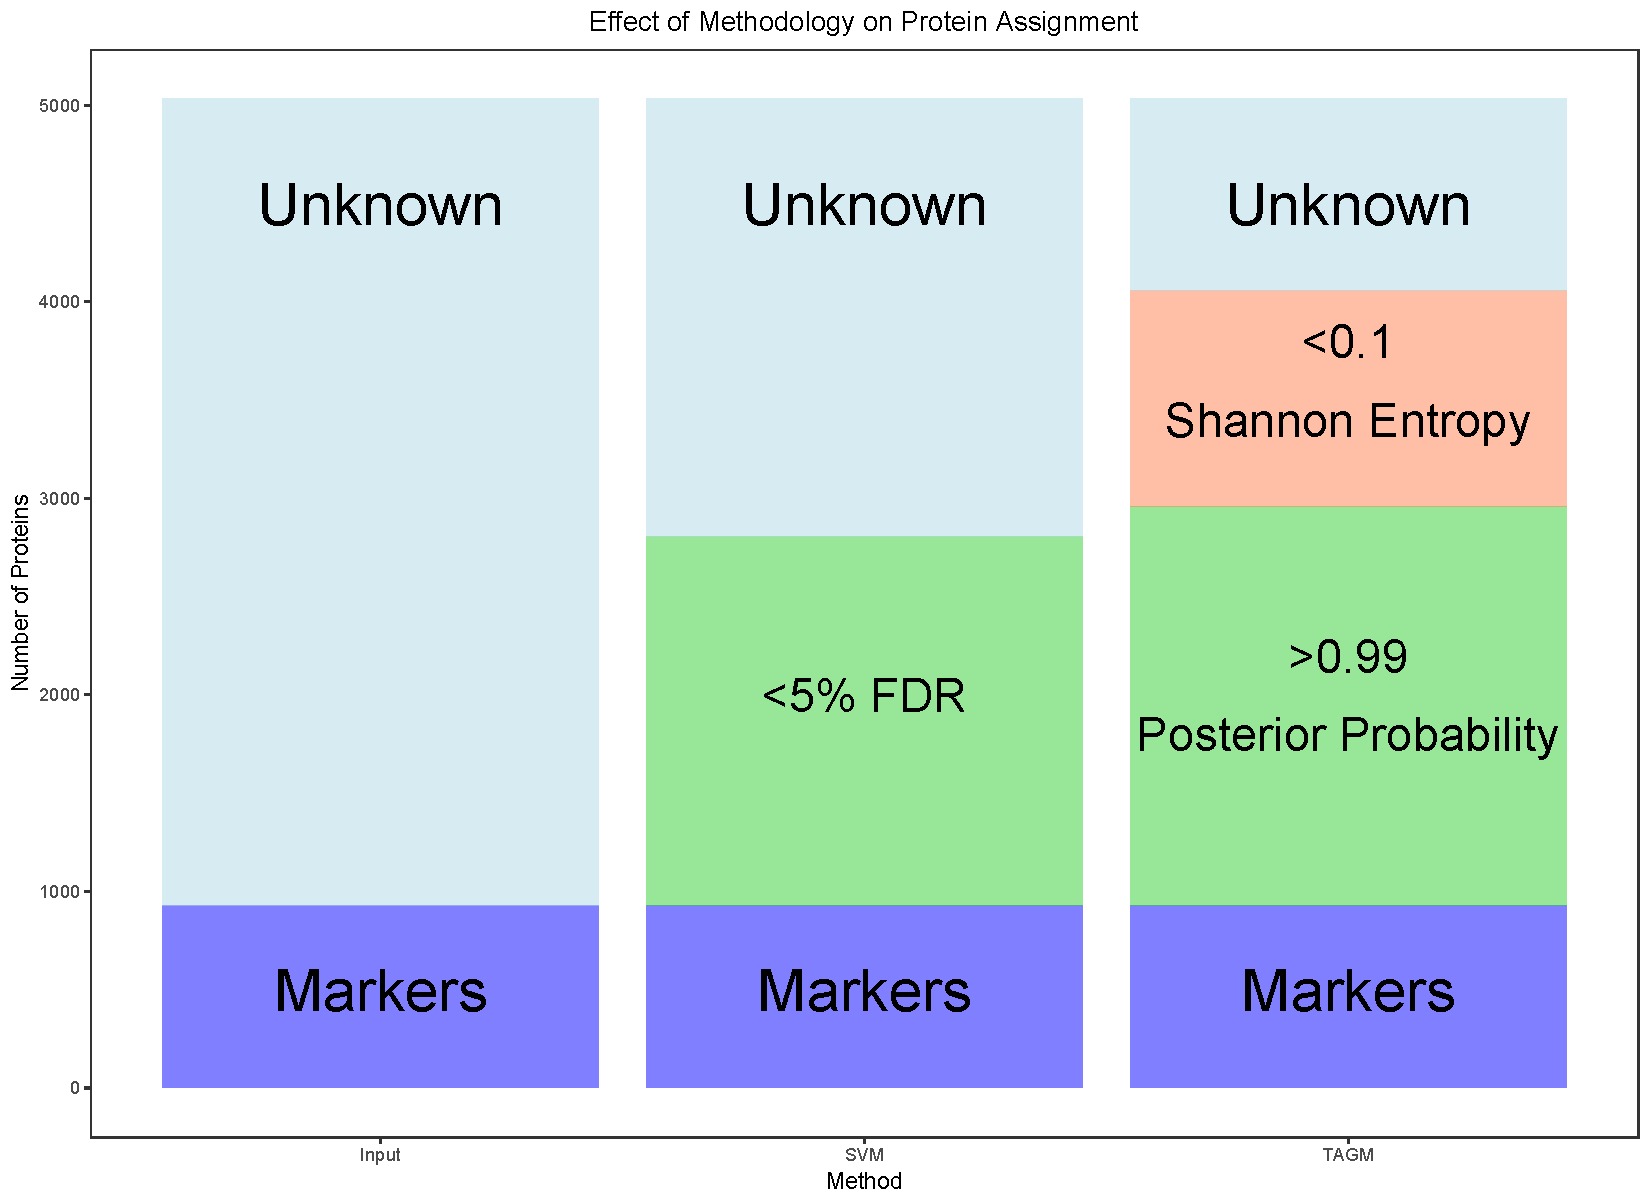
\includegraphics[width=.7\textwidth]{./figs/ConcludePlot.pdf}
\caption{The barplot demonstrates the effect of applying different
  methodologies on protein assignment when applied the mouse
  pluripotent embryonic stem cell data. Roughly 2000 proteins are
  classified using either SVM and TAGM-MCMC; however, TAGM-MCMC can
  draw additional conclusions about an extra 1000 proteins by
  quantifying uncertainty.}
\label{figure:ConcludePlot}
\end{figure}

\begin{figure}[!p]
  %% 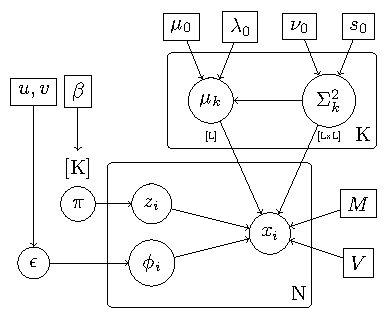
\includegraphics[width=8cm]{./figs/graphmodel2.pdf}
  \centering
  \caption{Plate diagram for TAGM model. This diagram specifies the
    conditional independencies and parameters in our
    model.}\label{plateDiagram}
\end{figure}

\clearpage

\section*{Supporting Information Legends}

\noindent Figure A: Plot of the log-posterior at each iteration of the
EM algorithm to demonstrate monotonicity and convergence

\bigskip

\noindent Figure B: Trace plots of the number of proteins allocated to
the known components in each of 6 parallel MCMC runs. Chain $4$ is
discarded because of lack of convergence. $600$ samples are retained
from remaining chains and pooled.

\bigskip

\noindent Figure C: Gene Ontology over representation analysis on
outlier proteins - that is proteins allocated with less than
probability $0.95$. We analyse the enrichment of terms in the cellular
compartment, biological process, and molecular function ontologies. We
display the top 10 significant results in the dotplots.

\bigskip

\noindent Figure D: A heatmap representation of a contingency table
comparing allocation produced by MCMC and MAP methods with posterior
probability threshold set at $0.99$ for both methods.  The scale
ranges from 0 to 1 with values indicating the proportion of assigned
proteins to that sub-cellular location. Values along the diagonal
represent agreement between classifiers whilst other values represent
disagreement.  The allocations of proteins by both methods are in
strong agreement.

\end{document}
